% =====================================================================
% CogniHire: Auditing Résumé Claims Instead of Scoring Candidates
%
% Written to the format supplied by the project guide:
%   Bilal et al., "Impact of Intelligent Technologies on IoV Security:
%   Integrating Edge Computing and AI", ACM Comput. Surv. 58(15), Art. 385.
%
% BUILD:
%   pdflatex paper && bibtex paper && pdflatex paper && pdflatex paper
%
% NOTE: not compile-tested -- no TeX toolchain was available on the machine
% where this was written. Structure is validated; expect minor build fixes.
%
% acmart is required. If your distribution lacks it:
%   tlmgr install acmart      (TeX Live)
% or build on Overleaf, which ships it.
% =====================================================================

\documentclass[manuscript,screen,review=false]{acmart}

\AtBeginDocument{%
  \providecommand\BibTeX{{\normalfont B\kern-0.5em{\scshape i\kern-0.25em b}\kern-0.8em\TeX}}}

\setcopyright{cc}
\copyrightyear{2026}
\acmYear{2026}
\acmDOI{}
\acmJournal{CSUR}
\acmVolume{0}
\acmNumber{0}
\acmArticle{0}
\acmMonth{9}

\usepackage{booktabs}
\usepackage{pifont}
% Note: acmart already loads newtxmath, which defines \Bbbk. Adding amssymb on
% top of it raises "Command \Bbbk already defined". Nothing here needs amssymb,
% so it is deliberately not loaded.

% Presence / absence marks used in the comparison table, matching the
% template's convention.
\newcommand{\yes}{\textcolor{black}{\ding{51}}}
\newcommand{\no}{\textcolor{black}{\ding{55}}}

\graphicspath{{figures/}}

\begin{document}

\title{CogniHire: Auditing Résumé Claims Instead of Scoring Candidates}
\subtitle{Integrating Evidence Grounding, Machine Learning, and Deep Learning
for Accountable Technical Screening}

\author{Devesh S V}
\affiliation{%
  \institution{SRM Institute of Science and Technology}
  \department{Department of Computer Science and Engineering}
  \country{India}}
\email{deveshsv.386@gmail.com}

\begin{abstract}
Automated hiring systems overwhelmingly emit a \emph{score}: a scalar ranking a
candidate against others. Such scores resist explanation, give a candidate
nothing specific to contest, and carry growing regulatory exposure under New York
City Local Law 144, the Illinois Human Rights Act as amended by HB 3773, and the
European Union Artificial Intelligence Act. This article presents CogniHire, a
technical screening system built on the opposite premise. It audits the claims a
candidate makes about themselves, and it never scores the candidate. We use it to
examine how three technology families combine in accountable screening: evidence
grounding, machine learning (ML), and deep learning (DL).

We survey the architecture, failure landscape, and regulatory trajectory of
automated screening, then take each family in turn. Evidence grounding constrains
a language model to \emph{select} claim text and forbids it to \emph{author} any.
Measured across roughly 100{,}000 adversarial trials over 5{,}200 résumés, the
gate rejected every meaning-preserving paraphrase and every negation trap while
admitting every verbatim claim. For ML we report a nine-model, six-family
comparison under grouped cross-validation with significance testing, together
with a within-query diagnostic that separates matching ability from
candidate-level quality. Pooled metrics cannot make that separation. The
diagnostic overturned our own initial hypothesis. For DL we show that a plausible
authored similarity constant of 0.50 would have falsely rejected 41.4\% of
genuine identity matches, against 3.4\% at a threshold calibrated on Labeled
Faces in the Wild.

Two conclusions follow. The useful output of automated screening is an audit of a
candidate's claims, not a judgement of the candidate. And the recurring
engineering move is converting policy into structure: an import boundary that
fails the build, a type with no field to hold a fabricated value, a vocabulary
ban that forbids a composite score. We report a weak result and a rejected
component alongside the strong ones. A system that publishes only its successes
offers no evidence that it evaluates itself honestly.
\end{abstract}

\begin{CCSXML}
<ccs2012>
<concept><concept_id>10003456.10003457.10003580</concept_id>
<concept_desc>Social and professional topics~Employment issues</concept_desc>
<concept_significance>500</concept_significance></concept>
<concept><concept_id>10010147.10010257</concept_id>
<concept_desc>Computing methodologies~Machine learning</concept_desc>
<concept_significance>500</concept_significance></concept>
<concept><concept_id>10002951.10003227.10003351</concept_id>
<concept_desc>Information systems~Data mining</concept_desc>
<concept_significance>300</concept_significance></concept>
</ccs2012>
\end{CCSXML}

\ccsdesc[500]{Social and professional topics~Employment issues}
\ccsdesc[500]{Computing methodologies~Machine learning}
\ccsdesc[300]{Information systems~Data mining}

\keywords{Automated hiring, evidence grounding, claim verification, algorithmic
accountability, model comparison, benchmark critique, face verification,
threshold calibration, explainable AI}

\maketitle

% =====================================================================
\section{Introduction}
\label{sec:intro}
% =====================================================================

A technical interview ends and a form is filled in: \emph{``Strong communication.
Good Flutter knowledge. 8.7/10.''} Six months later the number is indefensible.
Nobody can reconstruct which answer moved it from 8.4 to 8.7. The candidate
cannot appeal it, because there is nothing specific to appeal. The recruiter
cannot defend it, because no record exists of what produced it. The number was
never knowledge; it was a compression of knowledge that discarded everything
needed to audit it.

Contemporary automated interview platforms largely reproduce this failure at
scale. They add throughput and consistency, and they keep the scalar. Faced with
criticism, the industry has mostly made the scalar more sophisticated, adding features, better models, and fairness post-processing. However, few have asked whether a scalar was the right output object at all.

\begin{figure}[t]
  \centering
  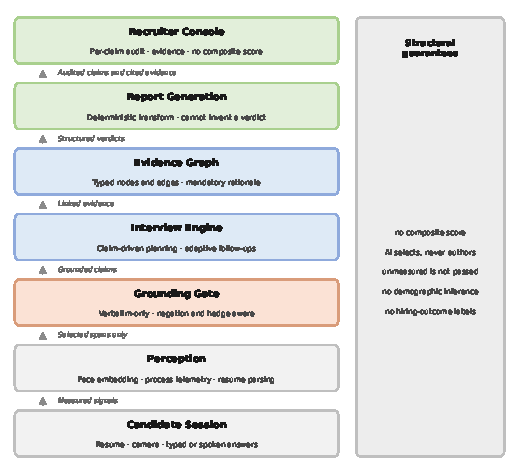
\includegraphics[width=\columnwidth]{fig01_dataflow.pdf}
  \caption{Data flow and component interactions in CogniHire. Evidence moves
  upward from the candidate session to the recruiter console; each transition
  narrows what the system is permitted to assert. The right-hand band lists the
  guarantees enforced structurally, not by convention
  (\S\ref{sec:integration}).}
  \label{fig:dataflow}
\end{figure}

This article takes the opposite position. The useful output of an automated
screening stage is an audit of the claims the candidate has made, not a
judgement of the candidate. A résumé is a set of assertions. Each assertion can
be probed, each probe yields evidence, and evidence supports a verdict about
\emph{the claim}. The verdicts, with their evidence attached, go to a human who
decides about \emph{the person}. Figure~\ref{fig:dataflow} shows the resulting
data flow.

The reframing is not only ethical positioning. It changes what the system must be
able to do, and more importantly what it must be \emph{unable} to do. It also
changes which technologies belong at which layer. Three families carry the load.
Evidence grounding constrains generative extraction so that a model may select a
candidate's own words but never compose new ones. Machine learning measures
properties of the accumulated evidence. Deep learning supplies perception: face
embedding for identity continuity, sentence encoding for semantic comparison.
We take each in turn, and \S\ref{sec:integration} asks what their combination
buys that none delivers alone.

\paragraph{Scope of this article.}
We survey the architecture, failure landscape, and regulatory trajectory of
automated candidate screening, and examine the integration of grounding, ML, and
DL within it. Where the literature supports a claim we cite it; where we have
measured something ourselves we report the measurement, the protocol, and the
uncertainty. The system described is deployed, and \S\ref{sec:deployment}
reports what deployment taught us, including three gaps we name openly.

\subsection{Key Research Questions}

This article addresses the following questions:

\begin{enumerate}
\item What distinct failure modes arise in automated candidate screening, and how
      do they differ from the failure modes of conventional information systems?
\item How does constraining a generative model to \emph{selection} rather than
      \emph{authorship} change the guarantees a screening system can offer, and
      at what measurable cost?
\item To what extent does the choice of machine-learning algorithm determine
      screening performance, once evaluation controls for leakage and multiple
      comparisons?
\item What does a pooled evaluation metric actually reward on a paired matching
      task, and can the components be separated?
\item How much does an authored constant differ from a calibrated one in a
      security-adjacent perception component, and how would anyone know?
\item What synergistic benefits emerge from integrating grounding, ML, and DL
      that none of the three provides in isolation?
\item How do regulatory instruments governing automated employment decisions map
      onto concrete architectural obligations?
\item Which open problems must be resolved before evidence-based screening can be
      deployed at scale, and which are research rather than engineering
      problems?
\end{enumerate}

\begin{figure*}[t]
  \centering
  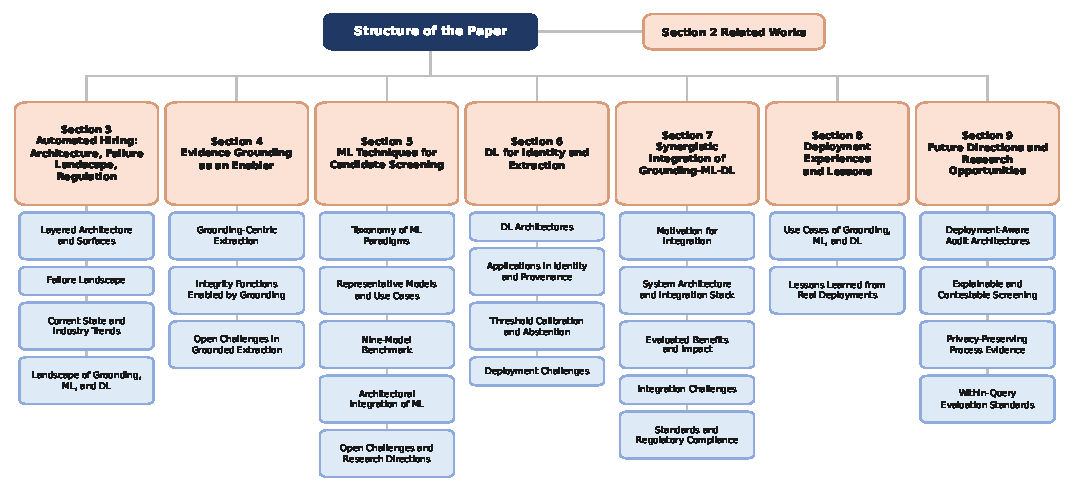
\includegraphics[width=\textwidth]{fig02_paper_structure.pdf}
  \caption{Overview of the paper structure.}
  \label{fig:structure}
\end{figure*}

\subsection{Structure of the Paper}

Figure~\ref{fig:structure} outlines the organisation. Section~\ref{sec:related},
\emph{Related Works}, reviews prior systems and surveys and positions this
study's contributions. Section~\ref{sec:landscape}, \emph{Automated Hiring:
Architecture, Failure Landscape, and Regulatory Trends}, discusses layered
models, the failure taxonomy, and the regulatory response.
Section~\ref{sec:grounding}, \emph{Evidence Grounding as an Enabler}, presents
the mechanism that makes the rest defensible. Sections~\ref{sec:ml}
and~\ref{sec:dl}, \emph{ML} and \emph{DL Techniques}, examine the learned
components. Section~\ref{sec:integration}, \emph{Synergistic Integration},
assesses the combined stack. Section~\ref{sec:deployment}, \emph{Deployment
Experiences and Lessons}, presents what shipping it taught us, and
Section~\ref{sec:future}, \emph{Future Directions}, identifies open challenges.
Section~\ref{sec:conclusion} concludes.

% =====================================================================
\section{Related Works}
\label{sec:related}
% =====================================================================

\subsection{Comparison of Existing Works}

Work adjacent to accountable candidate screening divides into four groups: audits of deployed hiring systems, methodological critiques of model comparison, studies of leakage and evaluation protocol, and technical work on the perception components that screening systems depend on. While each group is mature on its own terms, almost all of it treats these concerns in isolation, and the gaps we care about sit between them.
Table~\ref{tab:related} classifies the reviewed literature and states what this
work adds.

\begin{table*}[t]
\caption{Comparison of existing work on accountable screening and the research
gaps addressed here. \textbf{G}: evidence grounding; \textbf{ML}: machine
learning; \textbf{DL}: deep learning. \yes{} = present, \no{} = not present.}
\label{tab:related}
\small
\begin{tabular}{@{}llcccp{3.0cm}p{3.2cm}p{3.4cm}@{}}
\toprule
Ref (Year) & Type & G & ML & DL & Focus & Gaps & Improvements in this work \\
\midrule
\cite{raghavan2020hiring} (2020) & $\ast$ & \no & \yes & \no & Vendor bias-mitigation claims & No measurement of what the target actually is & Within-query test detects target substitution \\
\cite{dacrema2019progress} (2019) & $\ddagger$ & \no & \yes & \yes & Neural recommender baselines & Different domain; no grounding & Same protocol applied to screening \\
\cite{musgrave2020reality} (2020) & $\ddagger$ & \no & \no & \yes & Metric-learning evaluation flaws & No deployed system & Protocol plus a shipped system \\
\cite{demsar2006statistical} (2006) & $\dagger$ & \no & \yes & \no & Classifier comparison statistics & Method only & Applied end to end with power analysis \\
\cite{gorman2019splits} (2019) & $\ddagger$ & \no & \yes & \no & Standard-split fragility & NLP tagging domain & Grouped splits on a hiring corpus \\
\cite{kapoor2023leakage} (2023) & $\ast$ & \no & \yes & \yes & Leakage taxonomy across fields & No hiring instance & Leakage quantified on a hiring benchmark \\
\cite{grinsztajn2022tabular} (2022) & $\ddagger$ & \no & \yes & \yes & Trees vs.\ deep nets on tabular data & Benchmarks only & Spread shown to be noise-dominated here \\
\cite{deng2019arcface} (2019) & $\dagger$ & \no & \no & \yes & Angular-margin face embedding & Threshold left to the integrator & Threshold calibrated and reported \\
\cite{guo2022scrfd} (2022) & $\dagger$ & \no & \no & \yes & Efficient face detection & Detection only & Placed in a provenance pipeline \\
\cite{huang2007lfw} (2007) & $\oplus$ & \no & \no & \yes & Unconstrained verification benchmark & Not a hiring population & Used, with the mismatch stated \\
\cite{platt1999probabilistic} (1999) & $\dagger$ & \no & \yes & \no & Probability calibration & Classifier outputs & Applied to a similarity threshold \\
\cite{vovk2005algorithmic} (2005) & $\dagger$ & \no & \yes & \no & Distribution-free abstention & Theory & Abstention as a hard gate \\
\midrule
\textbf{This work} (2026) & --- & \yes & \yes & \yes & Grounded claim audit & --- & Unified grounding + ML + DL, measured \\
\bottomrule
\end{tabular}
\vspace{2pt}
\footnotesize
$\oplus$: benchmark/dataset; $\ast$: survey/review; $\ddagger$: applied research;
$\dagger$: framework/method.
\end{table*}

Four of these strands bear directly on what follows. Raghavan et al.~\cite{raghavan2020hiring}
surveyed vendors of algorithmic pre-employment assessment and drew attention to
the consequences of a vendor's choice of \emph{prediction target}, since the
fairness analysis that follows is conducted against the stated target rather than
the deployed one. That concern is central here, and although the paper offers no remedy for a misdescribed target, \S\ref{sec:ml} does supply a measurement procedure for detecting when the stated and deployed targets diverge.

A second strand re-ran published comparisons under controlled protocols and found
the reported progress did not survive. Ferrari Dacrema et
al.~\cite{dacrema2019progress} examined eighteen neural recommendation methods,
could reproduce only seven, and found six of those seven were often outperformed
by simple heuristics. Musgrave et al.~\cite{musgrave2020reality} reached an
analogous conclusion for deep metric learning. Our \S\ref{sec:ml} sits in this
tradition but differs in target. Instead of showing a complex method failing to beat a simple one, we find that \emph{no} method separates from any other, and
then trace why.

A third strand concerns evaluation protocol.
Demšar~\cite{demsar2006statistical} remains the standard reference for comparing multiple classifiers, and cautions specifically against reading a ranking off raw score differences. Gorman and Bedrick~\cite{gorman2019splits} showed system
rankings established on a single standard split frequently fail to reproduce
under regenerated splits. Kapoor and Narayanan~\cite{kapoor2023leakage} surveyed
machine-learning-based science across seventeen fields and documented leakage
affecting 294 papers. We adopt Demšar's protocol and quantify one of Kapoor and
Narayanan's leakage categories on a hiring benchmark.

Some crucial \emph{research gaps} follow from this comparison:

\begin{itemize}
\item \emph{Grounding is absent.} No reviewed work constrains generative
      extraction so that a model may select but not author. Extraction is treated as a generation problem and evaluated on fluency or coverage, whereas fidelity to the source document goes unmeasured.
\item \emph{Prediction targets go unverified.} Vendors and benchmarks alike state
      a target and evaluate against a pooled metric that cannot distinguish it
      from an easier correlate.
\item \emph{Authored constants persist.} Perception components ship with similarity thresholds chosen by reasoning and never measured, and the error stays invisible until someone runs a calibration study.
\item \emph{Isolation.} Grounding, ML, and DL are evaluated separately; no
      reviewed work reports what their integration measurably buys.
\end{itemize}

\subsection{Our Contributions}

\begin{enumerate}
\item A \textbf{claim-audit output model} replacing the composite score, with a
      four-valued verdict set that makes unmeasured evidence explicit instead of absent (\S\ref{sec:grounding}).
\item A \textbf{structurally enforced grounding constraint}, under which the
      model may select claim text but never author it. It is implemented as an
      import boundary that a continuous-integration test enforces, and
      \emph{measured} at 100\% paraphrase and negation-trap rejection across
      roughly 100{,}000 trials (\S\ref{sec:grounding}).
\item A \textbf{nine-model, six-family comparison} under grouped cross-validation
      with Friedman and Holm-corrected Wilcoxon testing, together with a
      synthetic positive control that establishes the protocol's statistical
      power (\S\ref{sec:ml}).
\item A \textbf{within-query ranking diagnostic} separating matching ability from
      entity-level quality on any paired benchmark with a recurring entity
      (\S\ref{sec:ml}).
\item An \textbf{empirical threshold calibration} showing that a plausible,
      documented, authored constant was wrong in a specific and quantified way
      (\S\ref{sec:dl}).
\item A \textbf{measurement type system} in which a failed measurement carries no
      value, so a failure cannot be silently coerced into a pass
      (\S\ref{sec:integration}).
\item A \textbf{deployed implementation} with the gaps between design and deployment named, not elided (\S\ref{sec:deployment}).
\end{enumerate}

\subsection{Literature and Corpus Review Process}

\begin{figure}[t]
  \centering
  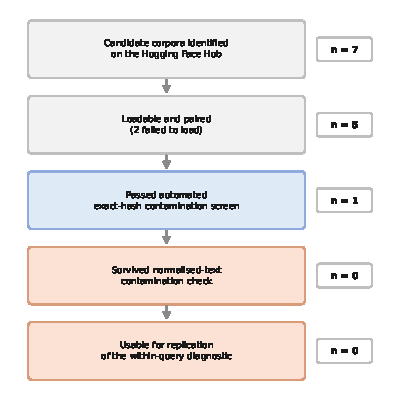
\includegraphics[width=0.86\columnwidth]{fig04_review_method.pdf}
  \caption{Replication-corpus screening. Counts are measured, not illustrative:
  seven candidate corpora were identified, five loaded and carried paired
  documents, one passed an exact-hash contamination screen, and none survived
  normalised-text verification (\S\ref{sec:ml}).}
  \label{fig:review}
\end{figure}

Two review processes underpin this article. For literature, every citation was
retrieved and read against a primary source before inclusion; the project has
previously had fabricated references caught in internal review, and the
verification rule was adopted in response. The bibliography is therefore smaller
than is conventional for a survey of this length. We prefer that to padding it
with work we have not read.

For datasets, Figure~\ref{fig:review} reports a screen of publicly hosted
résumé--posting corpora against three requirements: independence from the corpus
under study, recurring entities, and a binarisable fit label. The outcome is
reported in \S\ref{sec:ml} and is itself a finding.

% =====================================================================
\section{Automated Hiring: Architecture, Failure Landscape, and Regulatory Trends}
\label{sec:landscape}
% =====================================================================

\subsection{Layered Architecture and Surfaces}

An evidence-based screening system spans four surfaces, shown in
Figure~\ref{fig:layers}. A candidate-facing portal collects consent, résumé, and
session media. An inference service hosts the perception and learned components.
A persistence layer event-sources the session so it can be reconstructed turn by
turn. A recruiter-facing application renders the audit. The separation matters
because the guarantees this article describes are enforced at boundaries between
these surfaces rather than inside any one of them.

\begin{figure}[t]
  \centering
  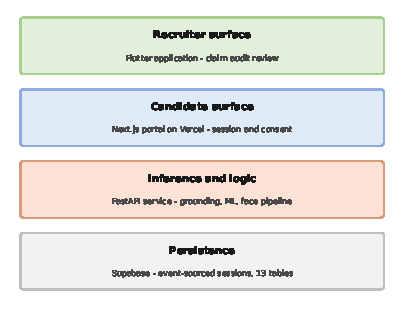
\includegraphics[width=\columnwidth]{fig05_layered_arch.pdf}
  \caption{Layered deployment architecture across the four surfaces.}
  \label{fig:layers}
\end{figure}

Session state is written to an append-only table with a sequence-assigning
database trigger. Question plans are deliberately \emph{not} persisted, so a plan
cannot be retrospectively edited to match an outcome --- a small design decision
that removes a whole category of post-hoc rationalisation.

\subsection{Failure Landscape}

Automated screening fails in ways that conventional information systems do not,
because its outputs are judgements about people and its inputs are difficult to
verify. Figure~\ref{fig:failures} organises the failure modes we encountered, and
Table~\ref{tab:threats} states their manifestations and defence implications.

\begin{figure*}[t]
  \centering
  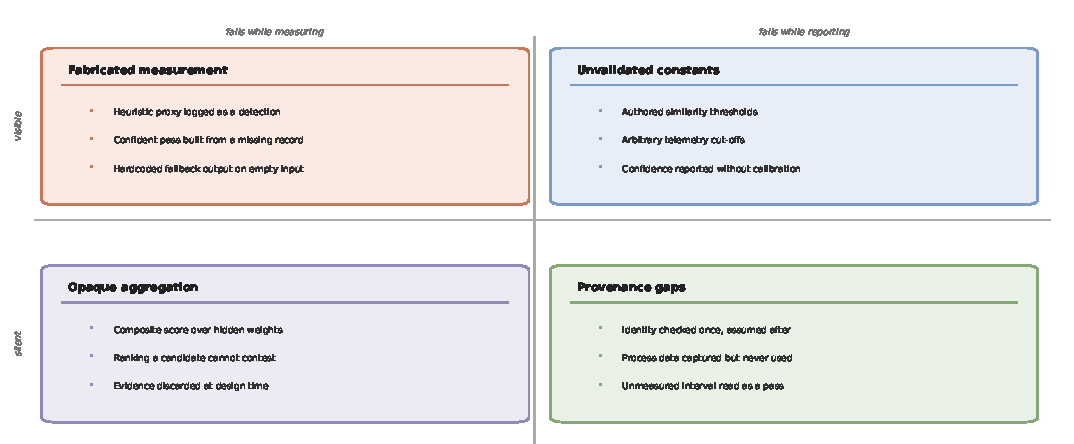
\includegraphics[width=\textwidth]{fig06_failure_landscape.pdf}
  \caption{Failure modes in automated candidate screening. The four families are
  not independent: fabricated evidence typically originates in an unvalidated
  constant and is concealed by opaque aggregation.}
  \label{fig:failures}
\end{figure*}

\begin{table*}[t]
\caption{Failure modes in automated screening, their manifestations, and defence
implications.}
\label{tab:threats}
\small
\begin{tabular}{@{}p{2.6cm}p{6.2cm}p{6.6cm}@{}}
\toprule
Failure mode & Manifestation & Defence implication \\
\midrule
Fabricated evidence & A heuristic proxy is logged under the label of a
measurement; a confident pass is returned when the underlying record is absent &
Measurements must be structurally distinguishable from inferences; absence must
have its own representation \\
Silent component outage & A model fails to load, a fallback fills the gap, and
the status is never surfaced & Health of every perception component must be
rendered where a human will see it \\
Unvalidated constants & A similarity or timing threshold is chosen by reasoning
and never measured & Security-adjacent constants require calibration studies with
reported error rates \\
Opaque aggregation & A composite score is produced from hidden weights and cannot
be explained or contested & Aggregation should be omitted where the downstream
decision is made by a human anyway \\
Provenance gaps & Identity is verified once at login and assumed thereafter &
Provenance must be continuous, and unmeasured intervals must be visible \\
Instruction injection & Text in a candidate document is interpreted as a
directive by a downstream model & Planning must consume typed structures, never
raw document text \\
\bottomrule
\end{tabular}
\end{table*}

The first two rows are not hypothetical. Section~\ref{sec:deployment} reports an
audit of a reference implementation in which both occurred simultaneously: an
object detector that never successfully loaded, a luminance heuristic that filled
the gap and logged its output as camera-verified detections, and a status string
reporting readiness that was never rendered anywhere.

\subsection{Current State and Industry Trends}

Table~\ref{tab:trad-vs-current} contrasts traditional screening practice with
current automated practice and states what each advance costs.

\begin{table*}[t]
\caption{Comparison of traditional and current automated screening solutions.}
\label{tab:trad-vs-current}
\small
\begin{tabular}{@{}p{2.4cm}p{4.4cm}p{4.4cm}p{4.2cm}@{}}
\toprule
Aspect & Traditional & Current & Advances and limitations \\
\midrule
Output object & Interviewer notes and a rating & Composite score or ranking &
Higher throughput; loses the evidence that justified it \\
Identity & Visual confirmation in person & One-time check at login &
Scales; assumes continuity that remote settings do not guarantee \\
Process evidence & Observed directly by the interviewer & Captured and filed for
retrospective review & Available for fraud investigation; not fed back into the
live interview \\
Consistency & Varies by interviewer & Uniform by construction & Removes one bias
source; can entrench another at scale \\
Explanation & Reconstructed from memory & Feature attributions over a score &
Post-hoc; explains the model, not the decision \\
Contestability & Conversation with the recruiter & Appeal against an opaque
number & Formally available, practically difficult \\
Auditability & Paper trail, incomplete & Logged, but of the score not the
evidence & Satisfies retention; not sufficient for a bias audit \\
\bottomrule
\end{tabular}
\end{table*}

\begin{figure}[t]
  \centering
  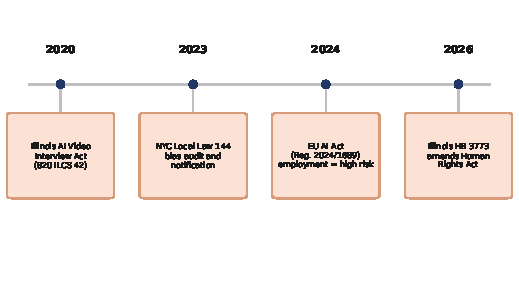
\includegraphics[width=\columnwidth]{fig08_regulatory_timeline.pdf}
  \caption{Regulatory instruments governing automated employment decisions.
  Dates are statutory effective dates.}
  \label{fig:regulation}
\end{figure}

Regulation is converging on explainability. Figure~\ref{fig:regulation} places
the four instruments that bear most directly on this system. The Illinois
Artificial Intelligence Video Interview Act took effect in 2020 and requires
notice and consent for AI analysis of interview video. New York City Local Law
144 requires bias auditing and candidate notification for automated employment
decision tools. The European Union Artificial Intelligence Act classifies
employment-related systems as high risk, with corresponding transparency and
human-oversight obligations. The Illinois Human Rights Act as amended by
HB 3773 constrains AI use in employment decisions from 2026.

These instruments share a direction: an automated employment decision must be
explicable and contestable. A system architected around a scalar faces a retrofit
that its architecture resists, because the explanatory information was discarded
at design time. Figure~\ref{fig:standards} summarises the practices that follow.

\begin{figure*}[t]
  \centering
  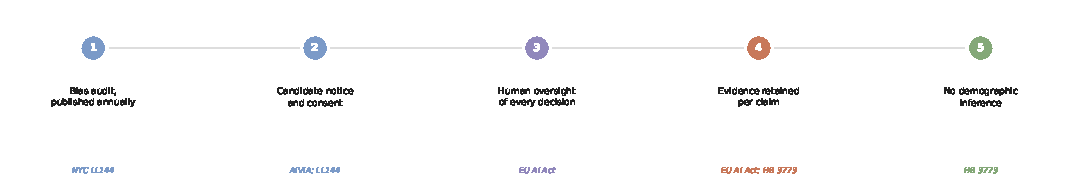
\includegraphics[width=\textwidth]{fig09_standards.pdf}
  \caption{Compliance practices implied by the instruments in
  Figure~\ref{fig:regulation}.}
  \label{fig:standards}
\end{figure*}

\subsection{Landscape of Grounding, ML, and DL}

Figure~\ref{fig:taxonomy} organises the technologies examined in the remainder of
this article. The division is not arbitrary: grounding governs what may be
\emph{asserted}, ML measures properties of \emph{evidence}, and DL supplies
\emph{perception}. Assigning a task to the wrong family is itself a failure mode
--- using a learned model where a rule is correct produces an unauditable
decision, and using a rule where measurement is required produces an unvalidated
constant.

\begin{figure*}[t]
  \centering
  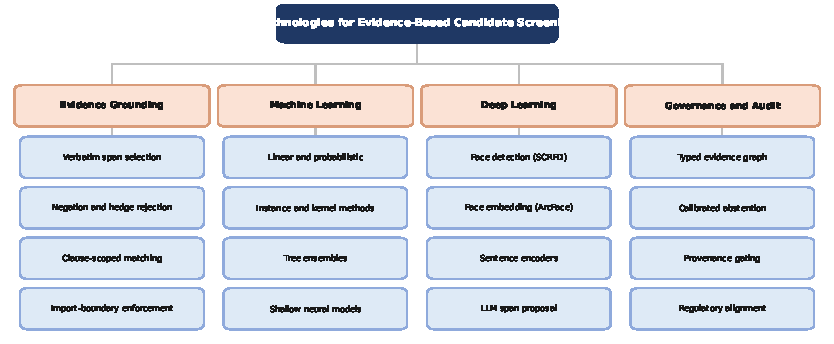
\includegraphics[width=\textwidth]{fig03_taxonomy.pdf}
  \caption{Taxonomy of technologies for evidence-based candidate screening.}
  \label{fig:taxonomy}
\end{figure*}

% =====================================================================
\section{Evidence Grounding as an Enabler}
\label{sec:grounding}
% =====================================================================

\subsection{Grounding-Centric Extraction}

The central mechanism of the system is a constraint on what a language model is
permitted to produce. Its rule: \textbf{a claim's text must be a verbatim
substring of the résumé.} The model's role is selection, not generation.

Naive substring matching is insufficient, and Figure~\ref{fig:gate} shows the
decision pipeline that replaces it. Beyond verbatim containment the gate
implements negation rejection, so that \emph{``I have not worked with
Kubernetes''} yields no Kubernetes claim despite containing the substring; hedge
rejection, so that \emph{``some exposure to Kafka''} is not a Kafka experience
claim; contrastive-conjunction splitting, so that \emph{``I used Django, but
never in production''} is split rather than truncated; and clause scoping, so
that matching occurs within clause boundaries rather than across them.

\begin{figure}[t]
  \centering
  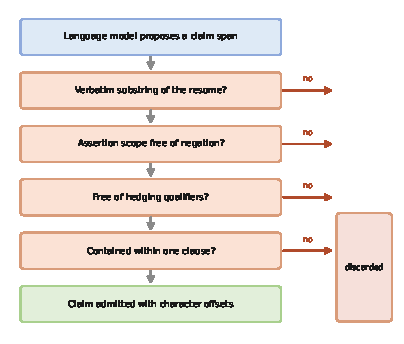
\includegraphics[width=0.92\columnwidth]{fig10_grounding_gate.pdf}
  \caption{The grounding gate as a decision pipeline. Any branch marked
  \emph{no} discards the proposed claim; nothing downstream sees it.}
  \label{fig:gate}
\end{figure}

\begin{figure*}[t]
  \centering
  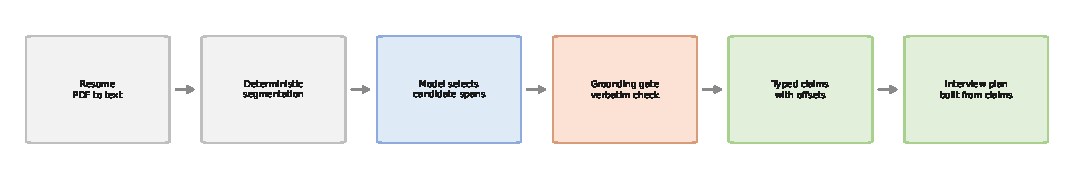
\includegraphics[width=\textwidth]{fig11_grounding_flow.pdf}
  \caption{End-to-end grounded extraction. Segmentation and normalisation remain
  deterministic; the model contributes span selection only.}
  \label{fig:groundflow}
\end{figure*}

\paragraph{Enforcement.}
The grounding module is forbidden from importing the AI module, and an
architecture test fails continuous integration if that import appears. The
guarantee is therefore a property of the build rather than of developer
discipline. Table~\ref{tab:grounding-adv} summarises what this buys.

\begin{table}[t]
\caption{Key advantages of evidence grounding.}
\label{tab:grounding-adv}
\small
\begin{tabular}{@{}p{2.3cm}p{5.1cm}@{}}
\toprule
Advantage & Basis \\
\midrule
Verifiable claims & Every claim is a substring with character offsets into the
source document \\
Injection resistance & Résumé text reaches the planner only as typed claims, so
an instruction in a document has no field to occupy \\
Auditable rejection & A discarded claim is discarded by a named rule, not by
model preference \\
Stable evaluation & The gate is deterministic, so its behaviour can be regression
tested at corpus scale \\
No fluency confound & Extraction quality is fidelity to the source, not the
plausibility of generated text \\
\bottomrule
\end{tabular}
\end{table}

\subsection{Integrity Functions Enabled by Grounding}

\begin{table*}[t]
\caption{Integrity functions enabled by grounding, and where each is exercised.}
\label{tab:grounding-features}
\small
\begin{tabular}{@{}p{3.0cm}p{5.6cm}p{6.4cm}@{}}
\toprule
Function & Mechanism & Application \\
\midrule
Claim provenance & Character offsets retained from extraction through to the
audit & A reviewer clicks a claim and lands on the candidate's own words \\
Prompt-injection defence & Planner consumes typed claims only & A résumé
containing an embedded instruction has no channel to the planner \\
Assertion-scope fidelity & Negation and hedge detection inside clause boundaries
& Denials and qualifications are not converted into claims \\
Quote fidelity in speech & Spoken-turn quotes must match the transcript verbatim,
including disfluency & An interviewer cannot attribute tidied speech to a
candidate \\
Non-fabrication of coverage & Unexamined claims carry an explicit verdict &
Absence of evidence is reported, not omitted \\
\bottomrule
\end{tabular}
\end{table*}

The last row deserves emphasis. The audit's verdict set is
\texttt{substantiated}, \texttt{notDemonstrated}, \texttt{contradicted}, and
\texttt{notExamined}, and the four are deliberately not orderable.
\texttt{notExamined} is load-bearing: without it an unprobed claim is simply
absent from the report, and absence reads as acceptance. Making non-measurement
explicit is what prevents an audit from being fabricated by omission.

\subsection{Measured Behaviour of the Gate}

The project's central claim is that the model selects but never authors. The
preceding subsections argue this structurally; this one measures it.

An offline deterministic harness drives the real pipeline modules read-only over
a corpus of 5{,}200 synthetic résumés spanning eight fields and four seniority
levels. No language-model key is required, so the result is reproducible by
anyone. Three quantities are measured across roughly 100{,}000 trials: the
verbatim true-positive rate, the paraphrase rejection rate, and the negation-trap
rejection rate. Figure~\ref{fig:gateresults} reports the outcome.

\begin{figure}[t]
  \centering
  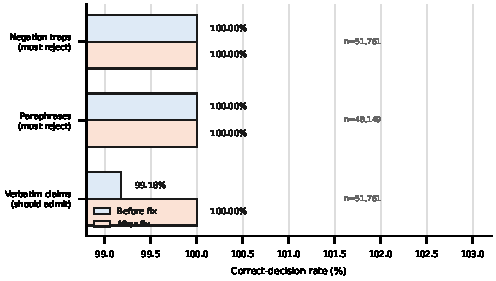
\includegraphics[width=\columnwidth]{fig07_grounding_gate_results.pdf}
  \caption{Grounding-gate evaluation before and after the clause-splitter fix
  described below. Trial counts are shown at right.}
  \label{fig:gateresults}
\end{figure}

\paragraph{The defect this surfaced.}
The initial run showed a 0.82\% false-rejection rate: 425 genuine claims wrongly
discarded. Every one contained a period-bearing token --- \texttt{Node.js},
\texttt{React.js}, \texttt{asp.net}, \texttt{Python 3.9} --- and \emph{zero}
occurred without one. The clause splitter treated a period, question mark, or
exclamation mark as a sentence terminal unconditionally, so
\emph{``\ldots using JavaScript, Node.js.''} split into \emph{``\ldots Node''}
and \emph{``js.''}, leaving a one-clause claim spanning two clauses where the
locator could never find it. The claim was then \emph{silently} rejected: no
error, no diagnostic, just an absent claim.

The fix constrains a terminal to count only when followed by whitespace or
end-of-string. A real sentence terminal always is; the period between two word
characters never is. Crucially, keeping dotted tokens whole makes clauses
\emph{longer}, which widens negation scope rather than narrowing it, so the fix
cannot weaken the guard --- and the measured before/after confirms it, with both
rejection rates unchanged at exactly 100\%.

This is a failure mode worth naming: the bug was \emph{silent}. Nothing crashed
and no test failed; claims simply went missing. Only a corpus-scale evaluation
with an explicit true-positive metric could surface it, which is an argument for
measuring the properties you claim rather than only testing the paths you wrote.

\paragraph{Honest scope.}
The corpus is synthetic and produced by a single generator, so 100\% extraction
coverage is an artifact of that format and is \emph{not} claimed as a general
result. The defensible claim is narrower and concerns the safety mechanism: the
gate rejected 100\% of model-style paraphrases and negation traps across roughly
100{,}000 trials while admitting 100\% of verbatim claims.

\subsection{Open Challenges in Grounded Extraction}

\begin{table}[t]
\caption{Future directions for grounded extraction and their expected impact.}
\label{tab:grounding-future}
\small
\begin{tabular}{@{}p{2.2cm}p{5.2cm}@{}}
\toprule
Direction & Expected impact \\
\midrule
Compositional claims & Extracting technology, artefact, metric, and agency as
typed relations rather than as a single span \\
Multilingual scope & Negation and hedge detection currently assume English clause
structure \\
Discontiguous spans & Some true claims are expressible only across
non-contiguous text; a discontiguous grounding relation would admit them without
loosening the gate \\
Speech grounding & Applying the constraint to spoken turns requires treating the
transcript as the source of truth, with its own error rate \\
\bottomrule
\end{tabular}
\end{table}

The gate's principal cost is recall on claims a résumé expresses across a
sentence boundary. Tightening that without loosening the safety property is the
main open problem in this component.

% =====================================================================
\section{Machine Learning Techniques for Candidate Screening}
\label{sec:ml}
% =====================================================================

\subsection{Taxonomy of ML Paradigms in Screening}

Machine learning enters an evidence-based screening system in exactly one place:
measuring properties of the evidence a session has accumulated. It does not
decide, and it is not trained on hiring outcomes. That restriction is what makes
the remainder of this section a measurement problem rather than a prediction
problem about people. Table~\ref{tab:ml-paradigms} states the paradigms and where
each is admissible.

\begin{table*}[t]
\caption{ML paradigms in candidate screening and their admissibility under an
evidence-audit design.}
\label{tab:ml-paradigms}
\small
\begin{tabular}{@{}p{2.4cm}p{5.2cm}p{3.2cm}p{4.6cm}@{}}
\toprule
Paradigm & Typical screening use & Admissible here? & Reason \\
\midrule
Supervised, outcome-labelled & Predict hire / no-hire from historical decisions &
\textbf{No} & Inherits whatever the historical decisions encoded; this is the
failure the 2018 Amazon case made famous \\
Supervised, evidence-labelled & Predict whether a session gathered enough
material to judge a claim & Yes & Target is a property of the interview, not of
the person \\
Relational / matching & Score a résumé against a posting & With care & Pooled
metrics conflate matching with candidate ranking (\S\ref{sec:withinquery}) \\
Unsupervised & Cluster claims, deduplicate skills & Yes & Structural, no verdict
produced \\
Self-supervised & Capture-quality prediction from embedding stability & Yes & No
human annotation, no person-level label \\
Reinforcement learning & Adaptive question selection & Offline only & Online
exploration means deliberately asking a real candidate a question believed to be
poor \\
\bottomrule
\end{tabular}
\end{table*}

\subsection{Representative Models and Use Cases}

\begin{figure*}[t]
  \centering
  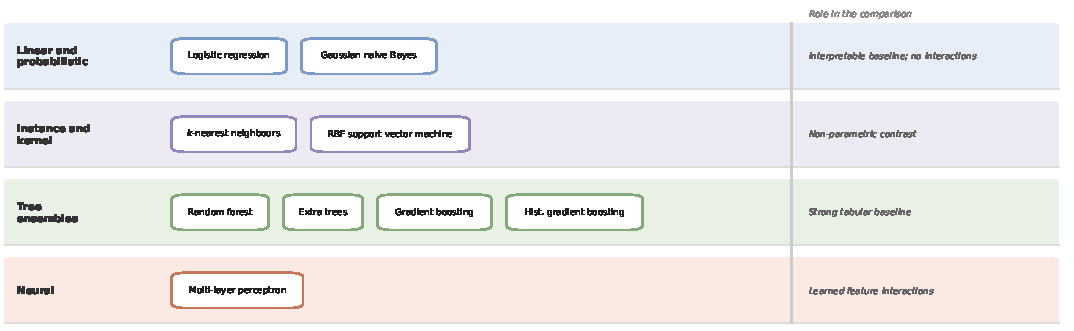
\includegraphics[width=\textwidth]{fig13_ml_roles.pdf}
  \caption{Model families evaluated in this work and the role each plays in the
  comparison.}
  \label{fig:mlroles}
\end{figure*}

Figure~\ref{fig:mlroles} shows the families compared, and
Figure~\ref{fig:mlevolution} places them against the evolution of screening
automation. Table~\ref{tab:ml-studies} summarises how the literature has applied
these families.

\begin{figure*}[t]
  \centering
  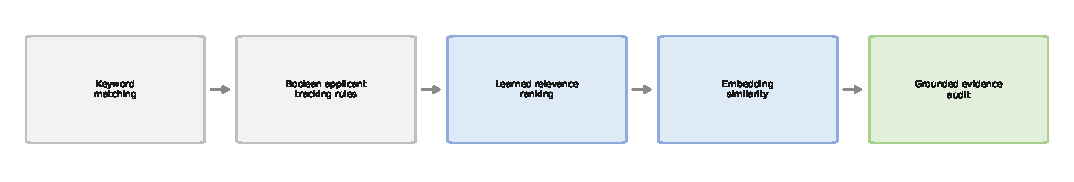
\includegraphics[width=\textwidth]{fig12_ml_evolution.pdf}
  \caption{Evolution of screening automation, from lexical matching to grounded
  evidence audit.}
  \label{fig:mlevolution}
\end{figure*}

\begin{table*}[t]
\caption{Methodological studies bearing on model comparison in screening-like
tasks, and the role each plays in this article's protocol.}
\label{tab:ml-studies}
\small
\begin{tabular}{@{}p{1.5cm}p{4.2cm}p{4.4cm}p{5.0cm}@{}}
\toprule
Refs & Technique / contribution & Focus & Role in this work \\
\midrule
\cite{demsar2006statistical} & Friedman test with post-hoc procedures &
Comparing many classifiers & Adopted as the significance protocol \\
\cite{nadeau2003inference} & Corrected variance for overlapping folds &
Generalisation-error inference & Motivates non-parametric paired tests \\
\cite{dacrema2019progress} & Reproduction under controlled protocol & Neural
recommenders vs.\ heuristics & Template for a null result that is informative \\
\cite{musgrave2020reality} & Evaluation-practice audit & Deep metric learning &
Precedent for attributing gains to protocol \\
\cite{gorman2019splits} & Randomly regenerated splits & Standard-split fragility
& Motivates ten grouped folds over one split \\
\cite{kapoor2023leakage} & Eight-type leakage taxonomy & ML-based science &
One category quantified in \S\ref{sec:splitscheme} \\
\cite{grinsztajn2022tabular} & Trees vs.\ deep nets, 45 datasets & Tabular
benchmarks & Context for family-level spread \\
\cite{pedregosa2011scikit} & Reference implementations & Toolkit & All nine
models are its estimators \\
\bottomrule
\end{tabular}
\vspace{2pt}
\footnotesize
Datasets, baselines, and evaluation metrics differ across the cited papers; the
table records each work's role, not a performance comparison.
\end{table*}

\subsection{A Nine-Model, Six-Family Comparison}
\label{sec:ninemodel}

We compare nine classifiers spanning six model families on a public
résumé--posting fit benchmark~\cite{resumejobfit2024} of 7{,}910 balanced pairs
drawn from 643 résumés and 351 postings. Every experiment uses ten-fold
\texttt{GroupKFold} grouped by job posting, so each fold's test postings are
absent from its training data. Two
quantities are fitted inside each fold on training rows only --- the IDF corpus
statistics and the feature scaler --- because fitting either over the pooled
corpus would leak the test fold's term distribution into training. Identical fold
assignments are reused across every model, so all comparisons are paired.

Models run at fixed modest hyper-parameters with no per-model tuning budget;
\S\ref{sec:tuning} tests whether that choice matters. Scale-sensitive models
receive standardised features and tree ensembles receive raw features, since
standardising a scale-invariant model would compare preprocessing rather than
algorithms.

\begin{table*}[t]
\caption{Nine classifiers on résumé--posting fit, ten-fold \texttt{GroupKFold} by
posting. Efficiency columns are per-fold means.}
\label{tab:ninemodel}
\small
\begin{tabular}{@{}lcccrrrr@{}}
\toprule
Model & AUROC & Accuracy & Macro F1 & ECE & Fit (s) & Latency ($\mu$s/row) & Size (KB) \\
\midrule
MLP                      & \textbf{0.696 $\pm$ 0.031} & 0.634 $\pm$ 0.021 & 0.658 $\pm$ 0.038 & 0.057 & 0.44 & 0.5 & 74.7 \\
Gradient boosting        & 0.689 $\pm$ 0.028 & \textbf{0.636 $\pm$ 0.024} & 0.655 $\pm$ 0.041 & 0.047 & 2.44 & 1.9 & 393.3 \\
Random forest            & 0.688 $\pm$ 0.030 & 0.628 $\pm$ 0.026 & 0.647 $\pm$ 0.042 & 0.047 & 0.59 & 88.2 & 24{,}732.6 \\
SVM (RBF)                & 0.686 $\pm$ 0.028 & 0.635 $\pm$ 0.023 & 0.651 $\pm$ 0.039 & 0.053 & 4.64 & 195.0 & 526.8 \\
Extra trees              & 0.685 $\pm$ 0.030 & 0.632 $\pm$ 0.026 & 0.641 $\pm$ 0.044 & \textbf{0.046} & 0.39 & 84.9 & 63{,}415.9 \\
$k$-NN                   & 0.680 $\pm$ 0.031 & 0.628 $\pm$ 0.029 & 0.639 $\pm$ 0.041 & 0.057 & 0.01 & 35.5 & 1{,}272.8 \\
Hist.\ gradient boosting & 0.679 $\pm$ 0.029 & 0.626 $\pm$ 0.020 & 0.643 $\pm$ 0.037 & 0.057 & 0.41 & 7.3 & 591.8 \\
Gaussian NB              & 0.667 $\pm$ 0.033 & 0.620 $\pm$ 0.027 & 0.633 $\pm$ 0.051 & 0.117 & 0.00 & 0.3 & 1.1 \\
Logistic regression      & 0.665 $\pm$ 0.022 & 0.616 $\pm$ 0.020 & 0.637 $\pm$ 0.042 & 0.052 & 0.01 & 0.2 & \textbf{0.9} \\
\midrule
\emph{Fixed-threshold baseline} & --- & \emph{0.513 $\pm$ 0.028} & --- & --- & --- & --- & --- \\
\bottomrule
\end{tabular}
\end{table*}

The nine span 0.031 AUROC from best to worst, and every model's fold-to-fold
standard deviation is of the same order as that entire spread. The Friedman test
rejects the hypothesis that all nine perform identically ($\chi^2 = 38.35$,
$p = 6.5 \times 10^{-6}$), so the models are not interchangeable --- but the
post-hoc picture is what governs a ranking claim. Comparing the leader against
each other model with a paired Wilcoxon signed-rank test over the ten folds and
applying Holm--Bonferroni correction, the leading model is \textbf{statistically
indistinguishable from all four tree ensembles}, separating only from the linear,
probabilistic, instance-based, and kernel baselines, where the largest effect is
three AUROC points.

A study reporting only the ranked table would license the claim ``the MLP is the
best model for résumé--job fit.'' The significance analysis does not support it.
Note also the non-monotonicity across metrics: the MLP leads on AUROC, gradient
boosting on accuracy, extra trees on calibration. Which model ``wins'' depends on
which column is placed first.

\paragraph{Establishing that the protocol has power.}
A comparison that finds no difference is uninformative unless the protocol can be
shown to detect a difference when one exists. We therefore constructed a
synthetic control with a pre-specified generative process --- twelve features,
eight carrying linear weights, one interaction term, one quadratic term, four
weightless, and a 7\% label-flip rate imposing a Bayes-optimal accuracy of 0.925
--- and ran it through the identical protocol. There the same nine models
separate decisively ($\chi^2 = 55.42$, $p = 3.7 \times 10^{-9}$), with the best
recovering 94.9\% of achievable accuracy.

\begin{figure*}[t]
  \centering
  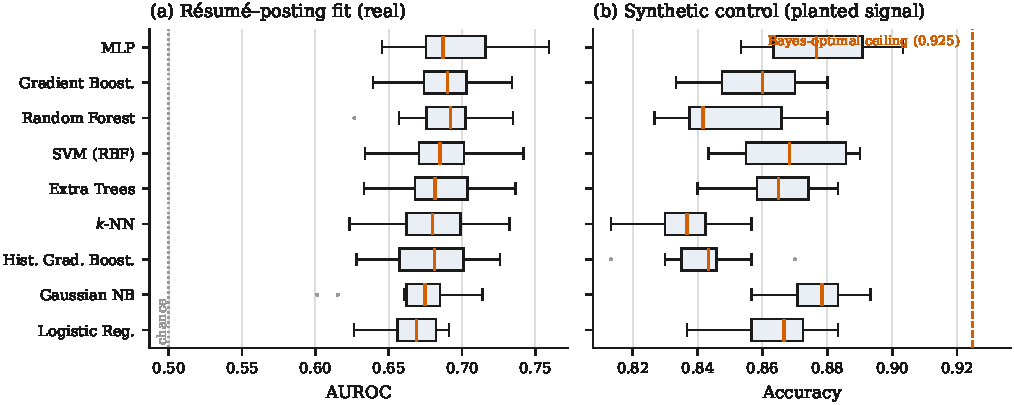
\includegraphics[width=\textwidth]{fig1_convergence_and_power.pdf}
  \caption{Per-fold distributions over ten grouped folds. \textbf{(a)} The nine
  models on the real screening task; the boxes overlap almost completely.
  \textbf{(b)} The same nine models, same folds, same code path, on the synthetic
  control, against its Bayes-optimal ceiling. Models appear in the same order in
  both panels. The contrast is the power analysis: an instrument reporting no
  difference in (a) is shown in (b) to be capable of reporting one.}
  \label{fig:power}
\end{figure*}

Figure~\ref{fig:power} places the two side by side.
\emph{The synthetic task is not a résumé task and its accuracy figures are not
screening performance.} It exists to characterise the protocol's power, and every
artifact it emits is flagged as synthetic. Its role is that of a positive control
in an assay: an instrument that reports nothing must be shown capable of
reporting something. The comparison licenses one inference --- when learnable
signal is present the protocol resolves it clearly, and on the résumé task it
does not --- so the null is a property of the task, not a limitation of the
study.

\subsection{Separating Matching from Candidate Quality}
\label{sec:withinquery}

A pooled metric rewards two distinct capabilities and cannot separate them. A
model that knows which \emph{résumés} tend to be labelled fit will score well,
and so will a model that knows which \emph{postings} a given résumé fits. Only
the second is matching.

Varying the representation while holding the protocol fixed localises where
performance comes from. A probe given only the résumé embedding --- which cannot
be matching, since it never sees the thing being matched against --- reaches
0.660 AUROC, 87\% of the best model's score and statistically indistinguishable
from a single cosine-similarity feature. Its mirror, given only the posting,
reaches 0.546, barely above chance. The best representation overall is plain
concatenation of the two embeddings at 0.755, which is to say that the
representation most enabling résumé recognition scores highest.

\begin{figure}[t]
  \centering
  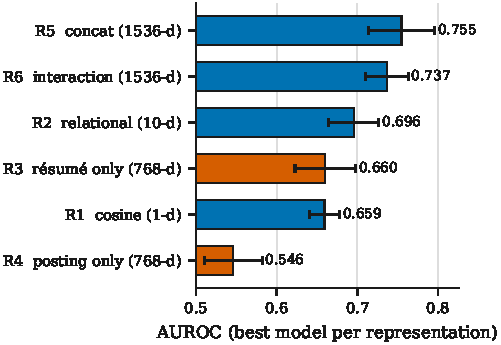
\includegraphics[width=\columnwidth]{fig2_representation_ablation.pdf}
  \caption{Best AUROC per representation, identical folds throughout. The
  highlighted bars are one-sided probes that cannot be performing matching: one
  never sees the posting, the other never sees the résumé.}
  \label{fig:ablation}
\end{figure}

Figure~\ref{fig:ablation} shows the ordering. That evidence pointed us toward a
strong conclusion --- that the benchmark's labels were not relational at all ---
and a direct test refuted it. Decomposing
label variance shows \textbf{80.6\% is within-résumé}: the same résumé labelled
fit for one posting and not for another. To measure whether models access that
variance we restrict evaluation to pairs of rows sharing a résumé, one positive
and one negative, and ask whether the model ranks the positive posting higher.
Because both items share a résumé, every résumé-level property cancels exactly,
and chance is 0.5 by construction.

\begin{table}[t]
\caption{Pairwise ranking accuracy. Random forest, identical folds, chance
$= 0.5$, 4{,}112 within-résumé pairs.}
\label{tab:withinquery}
\small
\begin{tabular}{@{}lccc@{}}
\toprule
Representation & Between & Within & Binomial $p$ \\
\midrule
Relational (10-d)    & 0.6905 & \textbf{0.6333} & $3.8 \times 10^{-66}$ \\
Interaction (1536-d) & \textbf{0.7372} & 0.6240 & $2.0 \times 10^{-57}$ \\
\bottomrule
\end{tabular}
\end{table}

\begin{figure}[t]
  \centering
  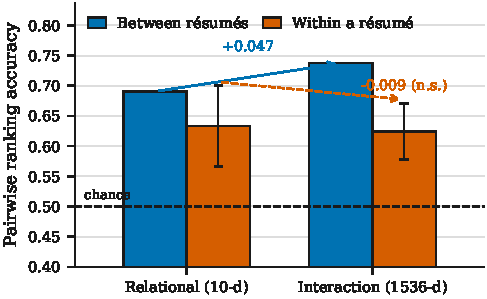
\includegraphics[width=\columnwidth]{fig03_matching_isolation.pdf}
  \caption{Pairwise ranking accuracy, chance $= 0.5$. Moving to the richer
  representation raises between-résumé ranking by 0.047 while leaving
  within-résumé matching unchanged ($-0.009$, $p = 0.445$).}
  \label{fig:withinquery}
\end{figure}

\textbf{Models do match.} Both representations rank within-résumé pairs well
above chance by every test applied. A model given one résumé and two postings
picks the fitting one roughly 63\% of the time.

\textbf{But the pooled gain does not come from matching.} Moving from the ten
engineered features to the 1536-dimensional interaction encoding raises
between-résumé ranking by $+0.047$ and pooled AUROC by $+0.041$, while
within-résumé matching changes by $-0.009$, which a paired Wilcoxon test over the
ten folds does not distinguish from zero ($p = 0.445$). We state this as
\emph{the gain does not transfer}, not as \emph{matching degrades}: the data
support the absence of an improvement, not the presence of a loss.

This is the section's central measurement. The representation change a
leaderboard would record as a clear improvement bought a better ordering of
résumés against each other and left the model's ability to tell which posting
suits a candidate where it was. Nothing in the pooled metric reveals which of the
two capabilities moved.

\paragraph{The diagnostic generalises.}
Nothing in the construction is specific to résumés. Any benchmark whose instances
are (entity, item) pairs with recurring entities --- candidate--job,
patient--treatment, user--item, student--question, query--document --- admits the
same test: condition on the entity, rank within it, compare against the pooled
number. It needs no extra labels and one pass over predictions already computed.
Where the two diverge, the pooled number is measuring something other than the
advertised capability. For algorithmic hiring specifically, this is the
measurement that distinguishes a system that ranks matches from one that ranks
people --- precisely the target substitution Raghavan et
al.~\cite{raghavan2020hiring} warn carries the ethical and legal weight.

\subsection{Robustness of the Comparison}
\label{sec:splitscheme}

\begin{table}[t]
\caption{Split-scheme comparison. Identical features and model throughout.}
\label{tab:splits}
\small
\begin{tabular}{@{}llc@{}}
\toprule
Scheme & Held out from training & AUROC \\
\midrule
S1 $k$-fold, no grouping & nothing & \textbf{0.7137 $\pm$ 0.016} \\
S3 GroupKFold by résumé  & every test résumé & 0.7032 $\pm$ 0.031 \\
S2 GroupKFold by posting & every test posting & 0.6894 $\pm$ 0.016 \\
\bottomrule
\end{tabular}
\end{table}

Two objections bear on the interpretation, and both are testable.

\emph{Does the protocol still permit résumé leakage?}
Table~\ref{tab:splits} varies only the splitting scheme. The ungrouped scheme a
conventional bake-off would use scores 0.024 AUROC above the posting-grouped
protocol we adopt, so the naive protocol inflates, modestly. But closing the
résumé channel does not collapse performance --- it raises it. We expected the
résumé-grouped scheme to fall sharply if the model's apparent skill were résumé
recognition; it scores 0.014 \emph{above} the posting-grouped scheme. A
strong-memorisation account predicts the opposite sign and is refuted. The
ordering instead tracks which side of the pair is novel, and generalising to a
new posting is the harder problem --- which matters in deployment, where every
new requisition presents exactly that condition.

\emph{Did binarising a three-class label destroy the signal?}
The cleanest available contrast, Good Fit against No Fit with the ambiguous
middle class removed, does \emph{not} exceed the binarisation used
(0.6810 vs.\ 0.6894), and its fold variance triples. Binarisation is not
concealing signal.

\subsection{Does Tuning Change the Conclusion?}
\label{sec:tuning}

The claim that nine models are statistically indistinguishable is vulnerable to
the objection that they were left untuned. We tested it with a design that could
have refuted the claim: a nested cross-validation whose outer loop is the same
ten folds and whose inner three-fold loop selects among eight configurations per
model --- an identical budget for every model, since an unequal budget compares
search effort rather than algorithms.

Tuning rescues no model. The largest gain across all nine is $+0.0077$ AUROC and
three models are marginally worse tuned than untuned, which is ordinary
nested-CV selection noise. The best-to-worst spread is essentially unchanged
($0.0311 \rightarrow 0.0317$), but the significance structure \emph{contracts}:
after Holm correction the tuned leader separates from only two of eight rivals
where the untuned leader separated from four. The two models that had been
significantly behind and gained most from tuning are no longer distinguishable
from the leader. Equal-budget tuning therefore leaves the ranking substantively
unchanged and weakens rather than strengthens the case that any model is best.

\subsection{Architectural Integration of ML}

\begin{figure}[t]
  \centering
  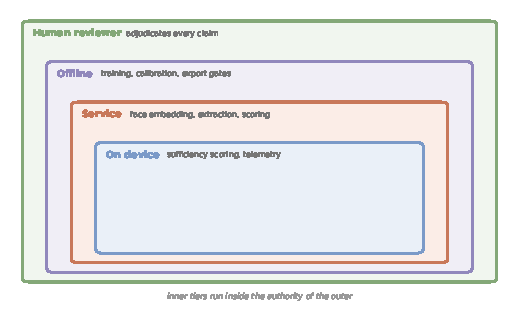
\includegraphics[width=0.92\columnwidth]{fig14_ml_tiers.pdf}
  \caption{Where each learned component runs. The human tier is not a fallback;
  it is the only tier that produces a decision about a person.}
  \label{fig:mltiers}
\end{figure}

Figure~\ref{fig:mltiers} shows placement. Two considerations drive it. Scoring
that must survive a network outage runs on-device, which is why the evidence
sufficiency model ships as exported coefficients rather than as a service call.
Components requiring model weights too large to ship run in the service. Training
and calibration are strictly offline and gated: the export refuses to write an
artifact unless held-out AUROC, calibration error, and Brier score all clear
stated bars, so a bad run produces no file rather than a quietly bad one.

\paragraph{Efficiency is decoupled from accuracy.}
Across the nine models, inference latency spans 0.2 to 195.0 $\mu$s per row --- a
factor of roughly 1{,}000 --- and serialised size spans 0.9 KB to 63.4 MB, a
factor of about 70{,}000. Predictive quality spans 0.031 AUROC.
Figure~\ref{fig:efficiency} shows the frontier, which is nearly flat. For an
interactive deployment the rational choice is therefore the cheapest model that
is not significantly worse, which here is a kilobyte of logistic-regression
coefficients rather than a 64-megabyte forest.

\begin{figure}[t]
  \centering
  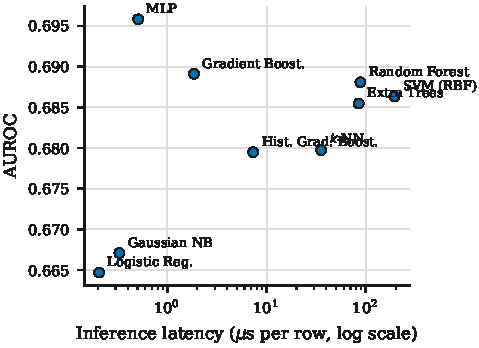
\includegraphics[width=\columnwidth]{fig4_efficiency_pareto.pdf}
  \caption{AUROC against inference latency (log scale). Three orders of magnitude
  of latency buy 0.031 AUROC, most of which is not statistically resolvable.}
  \label{fig:efficiency}
\end{figure}

\paragraph{More data would not close the gap.}
A learning curve over the same folds rises from 0.6514 AUROC at a tenth of the
training data to 0.6878 at all of it. Quadrupling the data from a quarter to full
buys 0.0204; doubling from half to full buys 0.0076. The curve is flattening well
below any useful operating point (Figure~\ref{fig:curve}), so the limitation is
not sample size and collecting more rows of this kind would not resolve it.

\begin{figure}[t]
  \centering
  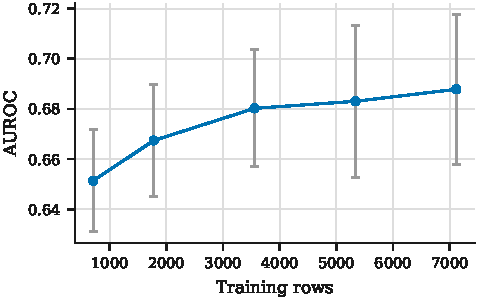
\includegraphics[width=\columnwidth]{fig5_learning_curve.pdf}
  \caption{Learning curve over the same ten folds. The curve flattens well below
  any useful operating point.}
  \label{fig:curve}
\end{figure}

\subsection{Open Challenges and Research Directions}

\begin{table}[t]
\caption{Challenges in ML for evidence-based screening.}
\label{tab:ml-challenges}
\small
\begin{tabular}{@{}p{2.0cm}p{5.4cm}@{}}
\toprule
Challenge & Impact and direction \\
\midrule
No independent corpus & Of seven public résumé--fit corpora screened, the
largest shares 100\% of its documents with the corpus under study and the
independent ones pair each résumé with exactly one posting, making the
within-query statistic undefined \\
Undocumented provenance & The benchmark carries no description, licence,
citation, or labelling procedure, so what a classifier trained on it has learned
cannot be stated \\
Evidence labels are costly & Annotating evidence sufficiency requires session
replay and multiple annotators; agreement is the model's performance ceiling and
must be reported \\
Representation ceiling & Changing representation moves AUROC about twice as far
as changing algorithm; effort is better spent there \\
\bottomrule
\end{tabular}
\end{table}

The first row is a finding rather than a limitation of effort. A benchmark whose
most-downloaded derivatives regenerate its labels by model and re-pair its
documents combinatorially is a benchmark whose apparent diversity is illusory:
work reporting evaluation across ``several résumé-fit datasets'' may be
evaluating repeatedly on one. We note also that an exact-hash contamination check
passed the contaminated corpus as clean, and only normalised matching exposed it.
Contamination audits should normalise before hashing and compare entity sets
rather than only pair sets, since re-pairing the same documents preserves
document overlap while destroying pair overlap.

% =====================================================================
\section{Deep Learning for Identity and Extraction}
\label{sec:dl}
% =====================================================================

\subsection{DL Architectures}

Two deep architectures carry load in this system, and neither is trained here.
Face detection uses SCRFD~\cite{guo2022scrfd}, whose contribution is
redistributing computation between backbone, neck, and head to detect small faces
efficiently. Face embedding uses ArcFace~\cite{deng2019arcface}, whose additive
angular margin loss produces highly discriminative 512-dimensional embeddings.
Both are consumed as pretrained components.

\begin{table*}[t]
\caption{Deep architectures in the pipeline: advantages, limitations, and use.}
\label{tab:dl-arch}
\small
\begin{tabular}{@{}p{2.4cm}p{4.4cm}p{4.4cm}p{4.2cm}@{}}
\toprule
Architecture & Advantage & Limitation & Use here \\
\midrule
SCRFD detector & Efficient across compute regimes; strong on small faces &
Detection only; no identity & Locating faces in webcam frames \\
ArcFace embedding & Angular margin yields separable identity geometry &
Threshold left to the integrator & 512-d embedding for identity continuity \\
Sentence encoder & Dense semantic comparison of free text & Similarity is not
entailment & Claim clustering and relational features \\
Language model (gated) & Fluent span proposal over messy documents & Will author
text if unconstrained & Proposes spans; the gate decides \\
\bottomrule
\end{tabular}
\end{table*}

\paragraph{Why the encoder is frozen.}
Retraining face recognition on a project-scale dataset would be strictly worse
than the pretrained model and would introduce demographic bias the project cannot
audit. The research question is not the encoder; it is what is done with the
embedding stream downstream. Relatedly, the vendor model pack ships an age and
gender classifier, and the loader specifies an allow-list that never loads it ---
a single argument a reviewer can verify, rather than a policy statement.

\subsection{Threshold Calibration and Abstention}

\begin{figure*}[t]
  \centering
  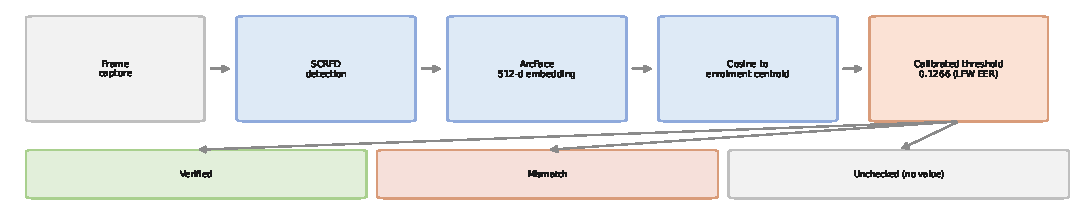
\includegraphics[width=\textwidth]{fig15_dl_identity.pdf}
  \caption{Identity pipeline. The result type is three-valued;
  \emph{Unchecked} carries a reason and no similarity value at all.}
  \label{fig:identity}
\end{figure*}

The system originally compared embeddings against an authored similarity
threshold of 0.50 --- a value arrived at by reasoning, documented honestly, and
flagged in its own source comment as uncalibrated. We replaced it with a measured
one. Using the Labeled Faces in the Wild benchmark~\cite{huang2007lfw}, an
equal-error-rate sweep on 2{,}200 training pairs and evaluation on 1{,}000
held-out pairs yields the results in Table~\ref{tab:calibration}. No weights are
trained; a single scalar is fitted.

\begin{table}[t]
\caption{Face-verification threshold before and after calibration on LFW.}
\label{tab:calibration}
\small
\begin{tabular}{@{}lcccc@{}}
\toprule
Threshold & FAR & FRR & Accuracy & AUC \\
\midrule
\textbf{0.1266} (calibrated) & 0.030 & \textbf{0.034} & \textbf{0.968} & 0.9785 \\
0.50 (authored) & 0.000 & \textbf{0.414} & 0.793 & --- \\
\bottomrule
\end{tabular}
\end{table}

\textbf{This is the article's most consequential single finding.} The prior
threshold was not arbitrary; it was reasoned, documented, and plausible. It was
also wrong in a way nobody could have known without measuring: it would have
falsely rejected \textbf{41.4\%} of genuine identity matches. In deployment,
roughly two in five legitimate re-verification checks would have failed --- and
because the system correctly refuses to treat an unmeasured check as a pass,
those candidates would have accumulated integrity flags for being themselves.
Calibration reduced false rejection by a factor of twelve at a false-acceptance
cost of 3.0\%. The lesson generalises beyond this component: in
security-adjacent systems, \emph{reasoned} and \emph{correct} are different
properties, and only one of them can be demonstrated.

\paragraph{Abstention as a hard gate.}
Figure~\ref{fig:identity} shows the three-valued result type.
\texttt{Unchecked} carries a reason and has \emph{no similarity field at all}. It
is not similarity 0.0, not null, not a default --- the value does not exist, so
no downstream comparison can read a failed measurement as a low-but-real one and
no serialisation can emit a number that was never measured. Selective prediction
of this kind is a hard constraint rather than a soft preference, in the spirit of
distribution-free abstention~\cite{vovk2005algorithmic}; a model that
\emph{usually} respects a safety constraint is a model that sometimes does not.

\paragraph{Stated limitation.}
LFW comprises public-figure photographs, not this system's candidate population.
The calibrated value is a defensible general threshold, not one validated on real
candidates, and population-specific recalibration requires consented candidate
data we have not collected.

\subsection{Deployment Challenges}

\begin{table}[t]
\caption{Challenges, impacts, and mitigations for DL components.}
\label{tab:dl-challenges}
\small
\begin{tabular}{@{}p{1.9cm}p{2.6cm}p{2.6cm}@{}}
\toprule
Challenge & Impact & Mitigation \\
\midrule
Population shift & Benchmark-calibrated thresholds may not transfer & Report the
mismatch; recalibrate under consent \\
Capture quality & Poor lighting widens within-session variance & Abstain rather
than mismatch \\
Silent model failure & A failed load can be masked by a fallback & Surface
component health in the UI; never substitute a heuristic \\
Embedding privacy & Face embeddings are invertible to recognisable faces &
Retain on-device, encrypted, with a deletion window \\
Demographic inference & Bundled classifiers infer protected attributes &
Allow-list modules; never load them \\
\bottomrule
\end{tabular}
\end{table}

% =====================================================================
\section{Synergistic Integration of Grounding, ML, and DL}
\label{sec:integration}
% =====================================================================

\subsection{Motivation for Integration}

Each family alone leaves a gap. Grounding guarantees that claims are the
candidate's own words but says nothing about whether a session gathered enough
evidence to judge them. ML measures evidence sufficiency but, without grounding,
would measure the sufficiency of text a model may have invented. DL supplies
identity continuity but produces no claim and no verdict. The combination closes
a loop that none closes alone, and Figure~\ref{fig:loop} shows its shape --- with
the human reviewer at the centre, because the loop deliberately terminates in a
person rather than in an aggregate.

\begin{figure}[t]
  \centering
  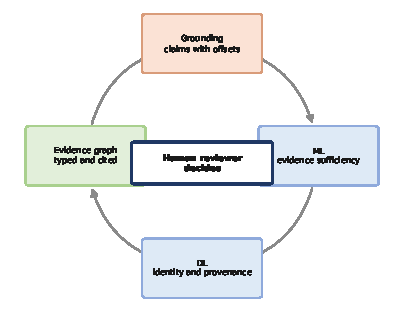
\includegraphics[width=0.92\columnwidth]{fig16_feedback_loop.pdf}
  \caption{The integrated loop. Every arrow carries typed, cited evidence; the
  reviewer is the only component that produces a decision about a person.}
  \label{fig:loop}
\end{figure}

\subsection{Evaluated Benefits and Impact}

\begin{table*}[t]
\caption{Key metrics before and after integration. Every row is a measured value
from this work, not an estimate.}
\label{tab:before-after}
\small
\begin{tabular}{@{}p{3.6cm}p{4.4cm}p{4.4cm}p{3.4cm}@{}}
\toprule
Metric & Before & After & Basis \\
\midrule
Identity false-rejection rate & 0.414 (authored threshold 0.50) &
\textbf{0.034} (calibrated 0.1266) & LFW, 1{,}000 held-out pairs \\
Paraphrase leakage & Unmeasured & \textbf{0 of 48{,}149} & Offline gate harness \\
Negation-trap leakage & Unmeasured & \textbf{0 of 51{,}761} & Offline gate harness \\
Verbatim admission & 99.18\% (425 wrongly rejected) & \textbf{100.00\%} &
Clause-splitter fix \\
Model-selection basis & Ranked table & Friedman + Holm-corrected pairwise &
Ten grouped folds \\
Matching vs.\ ranking & Conflated in one metric & Separated, 0.633 within-résumé
& 4{,}112 within-résumé pairs \\
Composite score & Present in comparable systems & \textbf{Absent by construction}
& Vocabulary ban fails the build \\
\bottomrule
\end{tabular}
\end{table*}

Table~\ref{tab:before-after} collects the measured effect of integration. Three
observations follow. First, the largest single improvement came not from a model
but from measuring a constant. Second, two rows read ``unmeasured'' before ---
the property was asserted rather than tested, which is the condition this article
argues is most common and least noticed. Third, the last row is a capability
\emph{removed}: the system cannot emit a composite score, and that absence is
enforced by a test.

\subsection{Architecture as Guarantee}

The recurring engineering move across all three families is converting a
\emph{policy} into a \emph{structure}.

\begin{table}[t]
\caption{Policies converted into structural guarantees.}
\label{tab:policy-structure}
\small
\begin{tabular}{@{}p{2.4cm}p{4.9cm}@{}}
\toprule
Policy & Structure \\
\midrule
AI must not author claims & Import boundary plus a CI architecture test \\
Unmeasured is not passed & A result type with no similarity field \\
No composite score & Vocabulary ban that fails the build \\
No demographic inference & Classifier module never loaded \\
No outcome labels & No such dataset and no code path to build one \\
Plans cannot be back-edited & Question plans are never persisted \\
Sessions must be reconstructible & Append-only event table with a sequencing
trigger \\
\bottomrule
\end{tabular}
\end{table}

Each row converts a claim that requires trust into one that can be checked in
seconds by someone who does not trust us. That is the property we would most like
other screening systems to adopt, independent of any of the specific technologies
in this article.

\subsection{Integration Challenges and Design Considerations}

\begin{table}[t]
\caption{Barriers to integration and mitigations.}
\label{tab:barriers}
\small
\begin{tabular}{@{}p{1.9cm}p{5.4cm}@{}}
\toprule
Barrier & Mitigation \\
\midrule
Interoperability & Typed contracts between surfaces; a failed measurement has its
own representation rather than a sentinel value \\
Lifecycle & Export gates refuse to write an artifact that misses its quality
bars; artifacts declare their own provenance and the loader rejects one that
misrepresents it \\
Latency budget & On-device scoring for anything on the interactive path; the
cheapest model that is not significantly worse \\
Compliance & Evidence retained per claim; no aggregate to explain because none is
produced \\
Drift & Thresholds and calibration are dated and re-measurable; nothing is
authored once and trusted indefinitely \\
\bottomrule
\end{tabular}
\end{table}

\subsection{Standards and Regulatory Compliance}

\begin{table*}[t]
\caption{Mapping regulatory obligations onto architectural mechanisms.}
\label{tab:compliance}
\small
\begin{tabular}{@{}p{3.4cm}p{5.4cm}p{6.4cm}@{}}
\toprule
Obligation & Instrument & Mechanism in this system \\
\midrule
Bias audit of the tool & NYC Local Law 144 & No composite score to audit; the
audited object is the per-claim verdict distribution \\
Candidate notification & NYC Local Law 144; Illinois AIVIA & Consent captured
per session with a recorded consent version \\
Human oversight & EU AI Act, Annex III high-risk & Report generation is a
deterministic transform containing no code that could emit a recommendation \\
Explanation and contestability & EU AI Act; HB 3773 & Every verdict carries its
evidence and character offsets into the candidate's own words \\
Non-discrimination & HB 3773; Illinois Human Rights Act & No demographic
inference, no outcome labels, no historical decision pattern to inherit \\
Traceability & All & Append-only event store; sessions reconstructible turn by
turn \\
\bottomrule
\end{tabular}
\end{table*}

The mapping in Table~\ref{tab:compliance} is possible only because the system
declines to produce an aggregate. A bias audit of a composite score must explain
the score; a bias audit of a claim audit examines the distribution of verdicts
and the evidence attached to each, which is a smaller and better-posed question.

% =====================================================================
\section{Deployment Experiences and Lessons}
\label{sec:deployment}
% =====================================================================

\subsection{Use Cases of Grounding, ML, and DL}

\begin{table*}[t]
\caption{Deployment case studies: where each technology family is exercised and
what it produced.}
\label{tab:cases}
\small
\begin{tabular}{@{}p{2.8cm}p{2.0cm}p{5.2cm}p{5.6cm}@{}}
\toprule
Case & Family & What was done & Core impact \\
\midrule
Corpus-scale gate evaluation & Grounding & 5{,}200 synthetic résumés, roughly
100{,}000 adversarial trials, run offline against real pipeline modules &
Surfaced a silent 0.82\% false-rejection defect invisible to the unit tests \\
Threshold calibration & DL & Equal-error sweep on LFW, 2{,}200 train and 1{,}000
held-out pairs & False rejection reduced from 0.414 to 0.034 \\
Nine-model comparison & ML & Ten grouped folds, Friedman plus Holm-corrected
Wilcoxon, synthetic positive control & Established that algorithm choice is not
the bottleneck on this task \\
Within-query diagnostic & ML & 4{,}112 within-résumé pairs, entity effects
cancelled by construction & Separated matching from candidate ranking; refuted
our own hypothesis \\
Sufficiency pipeline validation & ML & Planted-weight synthetic generator with
two weightless noise features & Pipeline recovered the planted structure and
correctly ignored the noise features \\
Independent security audit & All & Structured review of 17 public and 23
authenticated endpoints, 3 upload paths & 10 findings (5 high, 5 medium); 9
fixed, 1 mitigated \\
\bottomrule
\end{tabular}
\end{table*}

\subsection{Lessons Learned from Real Deployments}

The most instructive material came from auditing a reference implementation of a
comparable system, read in full before deciding what this project should inherit.
Its computer-vision core was sound and worth porting. Its decision layer, however, was largely fabricated, and the fabrications shared a single root cause.

\paragraph{A detector that never ran, and a heuristic that filled the gap.}
The object detector was configured with an invalid model name, so it threw on
every load and real detection never executed once. What filled the gap was a
luminance heuristic: if the left or right third of the frame deviated more than
60\% from mean brightness for three consecutive frames, it logged a phone or book detection, labelled \emph{camera verified}. A window, a desk lamp, or a light-coloured shirt was sufficient, and those fabricated events then fed an escalating penalty system. Compounding it, the load-failure handler set a status
string reading \emph{proctoring engine ready}, and that status was never rendered
anywhere, so a total detector outage was invisible.

\paragraph{A confident pass manufactured from missing data.}
The identity endpoint returned a verified result with a similarity of 98.7 and a
confidence of 0.98 when no enrolled face profile existed at all. The absence of a record produced a high-confidence pass, not an error.

\paragraph{Analysis that measured nothing.}
A résumé analyser substring-matched a fixed keyword list and, on zero matches,
returned a plausible-looking hardcoded skill list; its score was floored so an
unrelated résumé could never fall below a fifth of the scale. A speech-analytics
component took text rather than audio and derived fluency metrics from it.

\begin{table}[t]
\caption{Lessons carried into this system's architecture.}
\label{tab:lessons}
\small
\begin{tabular}{@{}p{2.1cm}p{5.3cm}@{}}
\toprule
Lesson & Architectural response \\
\midrule
A fallback that fabricates is worse than an outage & A failed measurement has its
own type carrying no value; nothing can substitute for it \\
Silent failure is the dangerous failure & Component health is surfaced where a
human sees it; corpus-scale evaluation with an explicit true-positive metric \\
Plausible output invites trust & Outputs are traceable to source spans, so
plausibility is checkable rather than persuasive \\
Hidden weights become verdicts & The composite score is removed, not improved \\
Reasoned is not correct & Security-adjacent constants require calibration studies
with reported error rates \\
\bottomrule
\end{tabular}
\end{table}

\begin{table}[t]
\caption{Where deep learning is and is not used, and why.}
\label{tab:dl-domains}
\small
\begin{tabular}{@{}p{2.0cm}p{5.4cm}@{}}
\toprule
Domain & Decision \\
\midrule
Face detection and embedding & Used, pretrained, frozen; genuinely a perception problem \\
Semantic comparison & Used for clustering and relational features; similarity is
not treated as entailment \\
Claim proposal & Used, but gated; the model never authors \\
Affect or emotion inference & \textbf{Not used.} No defensible accuracy on a
diverse candidate pool, and it maps onto disability, neurodivergence, and
cultural difference in expression \\
Demographic attributes & \textbf{Never loaded.} The bundled classifier is
excluded by an allow-list \\
Deception or cheating estimation & \textbf{Not built.} A learned cheating score
has no ground truth and cannot be calibrated \\
\bottomrule
\end{tabular}
\end{table}

Table~\ref{tab:dl-domains} records an argument worth stating explicitly. A
proposed live dashboard included confidence, stress, and eye-contact percentages
feeding back into question selection. We did not wire them in, and the reasoning
generalises: a stress percentage that silently changes which questions a
candidate is asked \emph{is} a hidden score, and one the candidate can neither
see nor contest. Every adaptive behaviour that dashboard promised is reachable from what the candidate \emph{said} --- observable, quotable, and defensible in a rejection conversation.

\subsection{Honest Position on Maturity}

Three gaps are stated openly here. Identity matching is implemented and
unit-tested but is currently only a presence gate on the production candidate
path, so the system does \emph{not} today perform continuous identity
verification. The face threshold is calibrated on a public benchmark rather than
on candidates. No structured recruiter validation interviews have been conducted,
which makes the premise that recruiters prefer a claim audit to a score the
project's largest untested assumption. The résumé--posting fit model reached
0.657 AUROC in earlier work and is \emph{not deployed}; no runtime module imports
it, and \S\ref{sec:ml} explains why that number is weak.

% =====================================================================
\section{Future Directions and Research Opportunities}
\label{sec:future}
% =====================================================================

\begin{table*}[t]
\caption{Research areas in evidence-based screening: core challenges and key
questions.}
\label{tab:research-areas}
\small
\begin{tabular}{@{}p{3.0cm}p{5.6cm}p{6.4cm}@{}}
\toprule
Research area & Core challenge & Key question \\
\midrule
Deployment-aware audit architectures & Continuous provenance without continuous
surveillance & How much identity assurance is obtainable from intermittent,
consented checks with explicit unmeasured intervals? \\
Explainable and contestable screening & Explanations that support appeal, not
just interpretation & Does a claim audit change human decisions relative to a
score, measured by inter-reviewer agreement? \\
Privacy-preserving process evidence & Keystroke and timing data are highly
identifying & Can within-session process deviation be measured on-device so only
derived scores leave the client? \\
Within-query evaluation standards & Pooled metrics conflate capabilities & Should
conditioning on the recurring entity become a reporting requirement for paired
benchmarks? \\
Benchmark provenance & Undocumented corpora beget undocumented derivatives &
What minimum provenance metadata should a hiring benchmark carry before it is
usable for published comparison? \\
Calibrated abstention & Choosing an operating point for ``unknown'' & What
abstention rate maximises usefulness while preserving honesty? \\
\bottomrule
\end{tabular}
\end{table*}

\subsection{Deployment-Aware Audit Architectures}

The immediate engineering task is wiring the calibrated matcher into the live
candidate session, which \S\ref{sec:deployment} records as not yet done. The
research question underneath it is more interesting: continuous verification and
candidate privacy pull in opposite directions, and the honest resolution is
probably not more surveillance but better accounting for intervals in which
nothing was measured.

\subsection{Explainable and Contestable Screening}

The project's core premise is untested: that a claim audit is more useful to a reviewer than a score. A controlled comparison of reviewers given an audit against reviewers given a score, measured by inter-reviewer agreement on identical sessions, would test it directly. We regard this as the single most valuable study the project
does not yet have, and note that it could refute the premise.

\subsection{Privacy-Preserving Process Evidence}

Process signals are informative and dangerous. Our position is that a deviation
in how an answer was produced should select a \emph{question}, never raise a \emph{flag}. The candidate's answer is the evidence. Whether that position survives contact with real candidates is, as yet, untested. Technically, the promising direction is
computing deviation on-device so that raw timings never leave the client and only a small number of derived scores are transmitted. That is a privacy property, not an optimisation.

\subsection{Within-Query Evaluation Standards}

\S\ref{sec:withinquery} showed that a representation change worth $+0.041$ pooled
AUROC delivered no measurable within-query improvement. The diagnostic costs one
pass over predictions already computed, needs no additional labels, and has a
fixed null of 0.5. We suggest reporting it alongside pooled metrics as a matter
of course for any paired benchmark with a recurring entity, and treating a
divergence between the two as information rather than as an anomaly to explain
away.

% =====================================================================
\section{Conclusion}
\label{sec:conclusion}
% =====================================================================

CogniHire replaces the composite hiring score with a per-claim audit. Claims are
extracted under a grounding constraint enforced by an architectural boundary
rather than by prompt discipline, probed in a live interview, and reported as verdicts traceable to evidence, including explicit statements about what was not measured. A human decides.

The methodological contribution is the repeated conversion of policies into
structures. ``The AI must not author claims'' becomes an import boundary with a
failing test. ``Unmeasured is not passed'' becomes a type with no field to hold a
fabricated value. ``No demographic inference'' becomes a module that is never
loaded. Each is verifiable by inspection in seconds, and none of them decays as attention moves elsewhere.

Three empirical findings stand out. The grounding gate rejected 100\% of
paraphrases and negation traps across roughly 100{,}000 adversarial trials while
admitting 100\% of verbatim claims, making ``the model selects, never authors'' a measured property, not a design aspiration. A carefully reasoned
similarity constant of 0.50 would have falsely rejected 41.4\% of genuine
identity matches; measurement reduced that to 3.4\%. And nine classifiers
spanning six families proved statistically indistinguishable at the top on a
public screening benchmark, while a within-query diagnostic showed that the
pooled metric's apparent gains came from ranking candidates rather than matching
them to roles.

That last finding deserves the final word, because it began as a different one.
The evidence initially indicated that the benchmark's labels were not relational
at all, and a direct test refuted it: four-fifths of the label variance is
within-résumé and models recover a real part of it. What survived was narrower: a decoupling between leaderboard progress and task progress that no pooled metric can reveal. We report the sequence rather than the conclusion alone,
because a diagnostic capable of distinguishing two hypotheses is only shown to
have that power when it actually overturns one.

We report a weak result and a rejected component alongside strong ones. A project
that publishes only its successes offers no evidence that it evaluates itself
honestly, and honest evaluation is what this system claims to provide to the
people it screens.

\section*{Data and Code Availability}

All analysis code, per-fold results, and figure sources accompany this article,
including the experiment scripts, the JSON reports they emit, and the
per-(model, fold) CSVs underlying every table and figure. The résumé--posting
corpus analysed is publicly available on the Hugging Face Hub; as
\S\ref{sec:ml} records, it carries no licence statement, and we analysed it as
distributed and redistribute none of it.

No human subjects were involved in the studies reported here. No résumé, job
posting, or candidate record was collected, contacted, or re-identified; the
face-verification study uses the public LFW benchmark~\cite{huang2007lfw}, and
the grounding evaluation uses a synthetic résumé corpus.

\section*{Declaration of Competing Interests}

The author declares no competing financial or non-financial interests. This work
received no external funding and was not commissioned, sponsored, or reviewed by
any vendor of hiring software.

\bibliographystyle{ACM-Reference-Format}
\bibliography{references}

\end{document}

